\documentclass[12pt,a4paper]{article}

% ─── Packages ─────────────────────────────────────────────────────────────────
\usepackage[T1]{fontenc}
\usepackage[utf8]{inputenc}
\usepackage{lmodern}
\usepackage[margin=1in]{geometry}
\usepackage{amsmath,amssymb,amsthm}
\usepackage{graphicx}
\usepackage{booktabs}
\usepackage{array}
\usepackage{caption}
\usepackage{subcaption}
\usepackage{float}
\usepackage{hyperref}
\usepackage{natbib}
\usepackage{setspace}
\usepackage{xcolor}
\usepackage{microtype}
\usepackage{parskip}
\usepackage{enumitem}
\usepackage{tabularx}
\usepackage{multirow}
\usepackage{makecell}

% ─── Hyperref Setup ───────────────────────────────────────────────────────────
\hypersetup{
  colorlinks = true,
  linkcolor  = blue!70!black,
  citecolor  = blue!60!black,
  urlcolor   = blue!70!black,
  pdftitle   = {A Comparative Study of Numerical Methods for European Option Pricing},
  pdfauthor  = {Chaithanya},
}

% ─── Typography ───────────────────────────────────────────────────────────────
\setstretch{1.15}
\setlength{\parindent}{0pt}
\setlength{\parskip}{8pt}

% ─── Custom Commands ──────────────────────────────────────────────────────────
\newcommand{\dollars}[1]{\$#1}
\newcommand{\method}[1]{\textit{#1}}
\newcolumntype{C}[1]{>{\centering\arraybackslash}p{#1}}
\newcolumntype{L}[1]{>{\raggedright\arraybackslash}p{#1}}
\newcolumntype{R}[1]{>{\raggedleft\arraybackslash}p{#1}}

% ─────────────────────────────────────────────────────────────────────────────
\begin{document}

% ─── Title Page ───────────────────────────────────────────────────────────────
\begin{titlepage}
  \centering
  \vspace*{1.5cm}
  {\LARGE\bfseries A Comparative Study of Numerical Methods\\[6pt]
  for European Option Pricing:\par}
  \vspace{0.5cm}
  {\large Black-Scholes, CRR Binomial Trees, Monte Carlo\\
  Simulation with Variance Reduction, and the\\
  Heston Stochastic Volatility Model\par}
  \vspace{1.5cm}
  {\large\bfseries Chaithanya\par}
  \vspace{0.4cm}
  {\normalsize Independent Researcher\par}
  \vspace{0.4cm}
  {\normalsize \href{https://github.com/Chaithanya5gif/Options-pricing-engine}%
    {\texttt{github.com/Chaithanya5gif/Options-pricing-engine}}\par}
  \vspace{1.5cm}
  {\normalsize June 2026\par}
  \vspace{1cm}
  \hrule
  \vspace{0.4cm}
  \textbf{Keywords:} option pricing, Black-Scholes, Heston model, Monte Carlo simulation,
  binomial tree, deep learning, implied volatility surface, LSTM, VAE, neural Greeks
  \vspace{0.4cm}
  \hrule
\end{titlepage}

% ─── Abstract ─────────────────────────────────────────────────────────────────
\begin{abstract}
\noindent
This paper presents a systematic, reproducible comparison of classical numerical
methods, stochastic volatility models, and modern deep learning approaches for
pricing European options.
Seven methodologies are implemented from scratch in Python and evaluated
head-to-head on 200~live SPY call options (June 2026).
We benchmark the Black-Scholes analytical formula, the Cox--Ross--Rubinstein
binomial lattice, Monte Carlo simulation with antithetic and control-variate
variance reduction, and the Heston (1993) stochastic volatility model—alongside
three deep learning architectures: a Multi-Layer Perceptron (MLP), an
LSTM-based volatility forecaster, and a Variational Autoencoder (VAE) for
implied-volatility surface generation.
Classical GBM methods cluster at MAE \$0.904 with near-identical accuracy;
the Heston model achieves MAE \$1.04 while being the only method that
structurally reproduces the empirical negative-skew implied-volatility smile
($\rho=-0.7$, IV range 17.3\%–23.0\%).
Deep learning architectures do not outperform Black-Scholes on point accuracy
for vanilla calls but solve structurally distinct problems.
All source code is publicly available.
\end{abstract}

\tableofcontents
\newpage

% ═══════════════════════════════════════════════════════════════════════════════
\section{Introduction}
% ═══════════════════════════════════════════════════════════════════════════════

Options pricing is a fundamental problem in quantitative finance.
\citet{BlackScholes1973} established the benchmark for pricing European options
under the assumption of constant volatility and continuous trading.
However, this foundational model has well-documented limitations.
The most prominent is the \emph{volatility smile} problem: empirical market data
consistently exhibits a negative skew---higher implied volatility for
out-of-the-money puts---which directly contradicts the Black-Scholes
assumption of log-normal asset price distributions.

Over the past five decades, researchers have developed numerical and stochastic
methods to address these shortcomings.
\citet{CRR1979} introduced the binomial lattice, which discretises time and
enables pricing of American-style options via backward induction.
\citet{Boyle1977} pioneered Monte Carlo simulation, offering a flexible
numerical approach for path-dependent exotic derivatives.
\citet{Heston1993} introduced a stochastic volatility model in which variance
follows a mean-reverting square-root diffusion correlated with the spot process,
providing the structural ability to price options consistently across strikes.

More recently, the literature has identified the potential of machine learning
to bridge the gap between classical theoretical limits and empirical realities.
As flexible universal function approximators, neural networks offer a promising
avenue to directly learn complex, non-linear pricing manifolds from market data
or to enhance existing models by forecasting dynamic parameters without relying
on rigid parametric assumptions.

In this context, this paper presents a systematic, reproducible comparison of
classical numerical methods, stochastic volatility models, and modern deep
learning approaches.
Our key contributions are:

\begin{enumerate}
  \item \textbf{Comprehensive Implementation.} We implement seven distinct option
    pricing methodologies from scratch in Python---ranging from classical
    Black-Scholes and CRR Binomial trees, to Euler-Maruyama Monte Carlo for the
    Heston model, to three distinct deep learning architectures (MLP, LSTM-BS
    Hybrid, and VAE).
  \item \textbf{Smile-Consistent Pricing Analysis.} We provide a detailed
    benchmarking of how each model handles the volatility smile, demonstrating
    quantitatively why flat-volatility models fail and how stochastic approaches
    (Heston) or generative ML models (VAE) successfully reconstruct the empirical
    volatility surface.
  \item \textbf{Rigorous Empirical Benchmarking.} We evaluate all models
    head-to-head on a live dataset of 200~SPY options across varying moneyness
    levels, offering a realistic assessment of the speed-accuracy tradeoff
    between fast analytical methods, accurate but computationally expensive
    numerical methods, and deep learning estimators.
\end{enumerate}

The remainder of this paper is structured as follows.
Section~\ref{sec:related} reviews related work.
Section~\ref{sec:foundations} outlines the mathematical foundations.
Section~\ref{sec:methodology} details the seven evaluated models.
Section~\ref{sec:results} presents empirical results and computational
benchmarks.
Section~\ref{sec:conclusion} concludes with directions for future research.

% ═══════════════════════════════════════════════════════════════════════════════
\section{Related Work}
\label{sec:related}
% ═══════════════════════════════════════════════════════════════════════════════

The mathematical pricing of options has evolved through several distinct phases.
The foundation was laid by \citet{BlackScholes1973}, who derived the first
closed-form analytical solution for European options under the assumption of
constant volatility.
Recognising the need to price American options, \citet{CRR1979} introduced the
binomial lattice model, which discretises time to allow early-exercise checking
via backward induction.
Simultaneously, \citet{Boyle1977} pioneered Monte Carlo simulation for options
pricing, offering a flexible numerical approach capable of handling complex,
path-dependent exotic derivatives, albeit at the cost of high computational
intensity.
To address the empirical reality of the volatility smile, \citet{Heston1993}
introduced a stochastic volatility model that allows variance to follow a
mean-reverting diffusion correlated with the spot process.

In recent years, the focus has shifted toward data-driven deep learning
approaches.
\citet{RufWang2020} provide a comprehensive literature review outlining how
neural networks are increasingly applied to both pricing and hedging.
Researchers have explored various network architectures for option pricing;
notably, \citet{ShvimerZhu2024} proposed a hybrid neural network model that
merges traditional mathematical bounds with data-driven flexibility, while
\citet{GrossKruger2025} confirmed the superior adaptability of deep learning to
market data in a detailed analysis against classical Black-Scholes and Bachelier
models.
More recently, \citet{Zheng2025} introduced ``Neural Jumps,'' an architecture
designed to capture discontinuous asset price movements, illustrating the
ongoing evolution of neural networks in financial modelling.
\citet{Gatheral2006} provides the practitioner's reference for the volatility
surface, against which all surface-generation models in this study are
conceptually grounded.

% ═══════════════════════════════════════════════════════════════════════════════
\section{Mathematical Foundations}
\label{sec:foundations}
% ═══════════════════════════════════════════════════════════════════════════════

\subsection{Black-Scholes Model}

The Black-Scholes (1973) framework prices a European call under risk-neutral
GBM dynamics.
Given spot price $S$, strike $K$, risk-free rate $r$, time to maturity $T$,
and constant volatility $\sigma$:
\begin{align}
  C &= S\,N(d_1) - K\,e^{-rT}\,N(d_2), \label{eq:bs}\\
  d_1 &= \frac{\ln(S/K) + \left(r + \frac{\sigma^2}{2}\right)T}{\sigma\sqrt{T}},
  \qquad d_2 = d_1 - \sigma\sqrt{T}. \nonumber
\end{align}
where $N(\cdot)$ denotes the standard normal CDF.
The analytical Greeks follow directly from differentiation of~\eqref{eq:bs}.

\subsection{Cox--Ross--Rubinstein Binomial Tree}

\citet{CRR1979} discretise the GBM into a recombinant binomial lattice with
parameters calibrated to match the continuous-time first two moments:
\begin{equation}
  u = e^{\sigma\sqrt{\Delta t}},\qquad d = \frac{1}{u},\qquad
  p = \frac{e^{r\,\Delta t} - d}{u - d}.
\end{equation}
Backward induction from the terminal payoff $\max(S_N - K,0)$ recovers the
present option value.
An early-exercise check at each node enables American-option pricing.

\subsection{Monte Carlo Simulation}

Under the risk-neutral measure, the terminal spot price is:
\begin{equation}
  S_T = S_0 \exp\!\left[\left(r - \tfrac{1}{2}\sigma^2\right)T
    + \sigma\sqrt{T}\,Z\right], \quad Z \sim \mathcal{N}(0,1).
\end{equation}
We implement two variance reduction techniques:
(i)~\textit{Antithetic Variates}—pairing each path with its negated
Brownian, halving the estimator variance; and
(ii)~\textit{Control Variates}—using the analytically known expected
asset price as a baseline correction, yielding a $2.62\times$ empirical
variance reduction on our test set.

\subsection{Heston Stochastic Volatility Model}

The Heston (1993) model extends GBM by making instantaneous variance $v_t$
itself a stochastic process:
\begin{align}
  dS &= r\,S\,dt + \sqrt{v}\,S\,dW_1, \label{eq:heston_s}\\
  dv &= \kappa(\theta - v)\,dt + \sigma_v\sqrt{v}\,dW_2, \label{eq:heston_v}\\
  &\quad\text{with}\quad \mathrm{Corr}(dW_1,dW_2) = \rho\,dt. \nonumber
\end{align}
The Feller condition $2\kappa\theta > \sigma_v^2$ ensures almost-sure positivity
of the variance process.
Negative $\rho$ generates the empirical left skew: OTM puts carry higher
implied volatility than OTM calls.
Parameters used throughout this study:
$\kappa=2$, $\theta=0.04$, $\sigma_v=0.3$, $\rho=-0.7$, $v_0=0.04$.

% ═══════════════════════════════════════════════════════════════════════════════
\section{Methodology}
\label{sec:methodology}
% ═══════════════════════════════════════════════════════════════════════════════

\subsection{Classical and Stochastic Methods}

\paragraph{Black-Scholes (BS).}
Closed-form analytical solution (Eq.~\ref{eq:bs}).
Five inputs: $S$, $K$, $T$, $r$, $\sigma$.
Executed in a single vectorised call; execution time $< 0.01$~ms per option.

\paragraph{CRR Binomial Tree.}
$N=200$ time steps, $O(N^2)$ backward induction.
Per-node early-exercise check enables American-style pricing.
Converges to Black-Scholes as $N\to\infty$.

\paragraph{Monte Carlo with Variance Reduction.}
$100{,}000$ paths with antithetic variates and control variates.
Standard error $\approx 0.057$ at $N=10{,}000$ paths (Table~\ref{tab:classic}).

\paragraph{Heston MC.}
Euler-Maruyama discretisation of Eqs.~\eqref{eq:heston_s}--\eqref{eq:heston_v}
with $N=252$ daily steps and $50{,}000$ antithetic paths for the smile plot;
$10{,}000$ paths with $N=63$ steps for evaluation speed.
Full-truncation scheme: $v_{t+\Delta t} = \max(v_t + \kappa(\theta-v_t)\Delta t
+ \sigma_v\sqrt{v_t\Delta t}\,Z_2,\;0)$.
Correlated Brownians: $Z_2 = \rho Z_1 + \sqrt{1-\rho^2}\,Z_3$.

\subsection{Deep Learning Architectures}

\paragraph{Multi-Layer Perceptron (MLP).}
Four fully connected layers (256-128-64-1) with ReLU activations and batch
normalisation, trained on $10^5$ synthetic BS prices via MSE loss.
Inputs: $S$, $K$, $T$, $r$, $\sigma$ (linear homogeneity scaling applied at
inference).
Training converges in $< 100$ epochs (Figure~\ref{fig:mlp_loss}).

\paragraph{LSTM-BS Hybrid.}
A two-layer stacked LSTM (hidden dim~64) ingests 60-day sequences of daily
log-returns and rolling historical volatility to forecast a scalar annualised
implied volatility.
The forecast $\hat{\sigma}$ is then substituted into the Black-Scholes formula,
ensuring an arbitrage-free final price.
The temporal context embeds recent market regime without requiring explicit
model recalibration.

\paragraph{Variational Autoencoder (VAE).}
The VAE learns a generative model of cross-sectional implied-volatility surfaces.
A flattened $M\times T$ IV grid is encoded into a latent space
$(\boldsymbol{\mu}, \log\boldsymbol{\sigma}^2) \in \mathbb{R}^{2\times d_z}$,
with $d_z=8$.
The decoder reconstructs the full surface via the reparameterisation trick.
Loss: $\mathcal{L} = \mathrm{MSE}(\hat{X}, X)
+ \beta\,D_{\mathrm{KL}}(\mathcal{N}(\boldsymbol{\mu},\,e^{\log\boldsymbol{\sigma}^2})
\;\|\;\mathcal{N}(\mathbf{0},\mathbf{I}))$
with $\beta=0.01$ (Figure~\ref{fig:vae_surfaces}).
At inference, the reconstructed surface is interpolated to the test strike/tenor
and fed into Black-Scholes for a final arbitrage-consistent price.

\paragraph{Neural MLP Greeks.}
In addition to pricing, we compute \emph{Neural Greeks} via automatic
differentiation through the MLP: $\Delta_{\mathrm{NN}} = \partial f/\partial S$,
$\mathcal{V}_{\mathrm{NN}} = \partial f/\partial \sigma$.
Figure~\ref{fig:neural_delta} compares $\Delta_{\mathrm{NN}}$ against the
analytical Black-Scholes $\Delta$ across strikes.

% ═══════════════════════════════════════════════════════════════════════════════
\section{Results}
\label{sec:results}
% ═══════════════════════════════════════════════════════════════════════════════

\subsection{Preliminary Benchmark: Classical Methods}

Table~\ref{tab:classic} confirms theoretical expectations on a single ATM
call ($S=100$, $K=100$, $T=1$, $r=0.05$, $\sigma=0.20$).

\begin{table}[H]
  \centering
  \caption{Classical method benchmark on a single ATM European call.}
  \label{tab:classic}
  \renewcommand{\arraystretch}{1.2}
  \begin{tabular}{lrrrrl}
    \toprule
    Method & Price (\$) & $|\Delta\text{BS}|$ & Std.\ Err & Time (ms) & Use Case \\
    \midrule
    Black-Scholes (exact)     & 10.45058 & ---     & ---     & 0.008 & European only \\
    CRR Binomial $N=200$      & 10.44059 & 0.00998 & ---     & 342.5 & European + American \\
    MC Control Variate (10k)  & 10.46574 & 0.01517 & 0.05707 & 0.23  & 2.62$\times$ var.\ reduction \\
    \bottomrule
  \end{tabular}
\end{table}

\begin{figure}[H]
  \centering
  \includegraphics[width=0.85\textwidth]{crr_benchmark.png}
  \caption{CRR Binomial tree convergence to the Black-Scholes price as $N$
    increases. The absolute pricing error decays at rate $O(N^{-1})$ in the
    smooth-payoff limit.}
  \label{fig:crr}
\end{figure}

\begin{figure}[H]
  \centering
  \includegraphics[width=0.85\textwidth]{mc_analysis.png}
  \caption{Monte Carlo convergence and variance reduction analysis.
    Control Variates (orange) achieve $2.62\times$ variance reduction versus
    the plain estimator (blue), reaching $\pm\$0.10$ accuracy with $\sim$2,500
    paths vs.\ $\sim$6,500 paths required without variance reduction.}
  \label{fig:mc}
\end{figure}

\subsection{Head-to-Head Comparison on Live SPY Options}

We evaluate all seven methods on a held-out test set of 200~SPY call options
drawn from live market data in June~2026
(SPY spot: \$736.70, risk-free rate: 5.25\%).
Options are stratified across five moneyness buckets (Table~\ref{tab:buckets}).
Ground-truth prices are the mid-market quote $(b+a)/2$.

\begin{table}[H]
  \centering
  \caption{Test-set stratification by moneyness.}
  \label{tab:buckets}
  \renewcommand{\arraystretch}{1.2}
  \begin{tabular}{lrr}
    \toprule
    Bucket     & Count & Moneyness $K/S$ Range \\
    \midrule
    Deep ITM   & 40    & $< 0.90$ \\
    ITM        & 41    & $[0.90,\;0.975)$ \\
    ATM        & 40    & $[0.975,\;1.025]$ \\
    OTM        & 40    & $(1.025,\;1.10]$ \\
    Deep OTM   & 39    & $> 1.10$ \\
    \bottomrule
  \end{tabular}
\end{table}

\begin{table}[H]
  \centering
  \caption{Head-to-head comparison of all seven methods on $n=200$ live SPY
    European call options. Bold indicates the best (lowest error or highest
    speed) in each column.}
  \label{tab:main}
  \renewcommand{\arraystretch}{1.3}
  \resizebox{\textwidth}{!}{%
  \begin{tabular}{lrrrrrrl}
    \toprule
    Method & MAE (\$) & RMSE (\$) & \%~within~5\% & MAE ATM & MAE OTM
      & Speed (ms/opt) & Best Use Case \\
    \midrule
    \textbf{Black-Scholes}     & 0.906 & 1.444 & 49.0\% & \textbf{0.379} & \textbf{0.019} & \textbf{0.01} & Fast European baseline \\
    \textbf{CRR Binomial N=200} & \textbf{0.905} & \textbf{1.443} & 47.5\% & 0.379 & 0.020 & 13.55 & American / early-exercise \\
    \textbf{Monte Carlo 100k}  & 0.904 & 1.446 & \textbf{50.5\%} & 0.381 & 0.020 & 1.23  & Exotic / path-dependent \\
    \textbf{Heston MC}         & 1.040 & 1.578 & 38.5\% & 0.455 & 0.146 & 18.21 & Stochastic vol / smile \\
    \textbf{LSTM-BS Hybrid}    & 1.048 & 1.490 & 41.0\% & 1.255 & 0.041 & \textbf{0.01} & Time-series vol forecasting \\
    \textbf{MLP Pricer}        & 6.658 & 7.311 & 12.5\% & 10.93 & 5.121 & 0.49  & Ultra-fast batch (in-dist.) \\
    \textbf{VAE-IV $\to$ BS}   & 2.476 & 3.148 & 25.5\% & 4.299 & 0.914 & 0.03  & IV surface interpolation \\
    \bottomrule
  \end{tabular}}
\end{table}

\begin{figure}[H]
  \centering
  \includegraphics[width=0.92\textwidth]{pricer_comparison.png}
  \caption{Box plots of absolute pricing errors for all seven methods across the
    200-option test set, stratified by moneyness bucket.
    The three classical GBM methods cluster within \$0.002 MAE of each other.}
  \label{fig:pricer}
\end{figure}

\begin{figure}[H]
  \centering
  \includegraphics[width=0.92\textwidth]{comparison_table.png}
  \caption{Radar chart summarising normalised performance across MAE, RMSE,
    speed, and percentage within 5\% for all seven methods.}
  \label{fig:radar}
\end{figure}

\subsection{Overall Performance}

The three classical GBM methods—Black-Scholes, CRR Binomial ($N=200$), and Monte
Carlo (100k paths)—cluster at overall MAEs of \$0.906, \$0.905, and \$0.904,
respectively (Table~\ref{tab:main}).
The spread among them is \$0.002—smaller than the bid-ask half-spread on most
test-set options—and statistically indistinguishable.
This convergence is theoretically expected: CRR converges to Black-Scholes as
$N\to\infty$, and Monte Carlo converges in expectation under GBM.
All three methods are fed the per-option market-implied volatility, so residual
errors reflect GBM structural limitations rather than differences between
pricing engines.

The Heston MC model achieves MAE \$1.04—15\% worse than vanilla Black-Scholes
on aggregate—but with a distinctive performance profile: Deep OTM MAE
\$0.016 (comparable to BS's \$0.019) and OTM MAE \$0.146 (substantially lower
than flat-vol methods in that regime).
Heston underperforms in ITM and Deep ITM ($2.15 and \$2.39 MAE) because the
fixed global skew parameters ($\rho=-0.7$, $\sigma_v=0.3$) are not calibrated
per-option; a full per-option calibration would materially reduce these errors.

The deep learning methods perform substantially worse on aggregate.
The VAE-IV $\to$ BS method achieves MAE \$2.48 (2.7$\times$ worse than BS);
the LSTM-BS hybrid registers MAE \$1.05; and the MLP produces MAE \$6.66
with only 12.5\% of options priced within 5\%.
These results establish a clear null result: on broad, stratified vanilla
European call pricing with available market IV, classical analytical and
numerical methods are not outperformed by any deep learning architecture tested.

\subsection{Performance by Moneyness}

Table~\ref{tab:bucket_winners} disaggregates performance by moneyness bucket.

\begin{table}[H]
  \centering
  \caption{Per-bucket winners and Heston MAE.}
  \label{tab:bucket_winners}
  \renewcommand{\arraystretch}{1.2}
  \begin{tabular}{lllr}
    \toprule
    Moneyness Bucket & Winning Method & Runner-Up & Heston MAE (\$) \\
    \midrule
    Deep ITM  & CRR Binomial N=200 & Black-Scholes & 2.385 \\
    ITM       & LSTM-BS Hybrid     & Black-Scholes & 2.145 \\
    ATM       & Black-Scholes      & CRR Binomial  & 0.455 \\
    OTM       & Black-Scholes      & CRR Binomial  & 0.146 \\
    Deep OTM  & Black-Scholes      & CRR Binomial  & 0.016 \\
    \bottomrule
  \end{tabular}
\end{table}

For OTM and Deep OTM options, where absolute prices are small, all methods
produce low absolute errors and ranking differences are negligible.
The competition is most meaningful in the ATM and ITM regions.
At ATM, Black-Scholes achieves MAE \$0.379 while the LSTM-BS hybrid is the
clear underperformer at MAE \$1.255—$3.3\times$ worse than BS—because a scalar
volatility forecast is structurally unable to reproduce the IV smile at different
strikes.
The MLP pricer degrades uniformly across all buckets: trained on synthetic data
with $S \in [50, 150]$ and deployed on SPY at \$736.70, the linear homogeneity
scaling trick only partially mitigates out-of-distribution domain shift.

\subsection{Computational Efficiency}

The speed hierarchy spans five orders of magnitude
(Figure~\ref{fig:pricer}, right panel).
Black-Scholes and LSTM-BS (post-training) both execute in \textbf{0.01~ms} per
option—consistent with their closed-form structure.
VAE-IV requires \textbf{0.03~ms}, the MLP \textbf{0.49~ms}, Monte Carlo
\textbf{1.23~ms}, CRR \textbf{13.55~ms}, and Heston MC \textbf{18.21~ms}—
roughly $1{,}820\times$ slower than Black-Scholes.
For real-time Greeks computation across a large options book, Heston at 18~ms
and CRR at 13.5~ms are prohibitive; Black-Scholes remains the dominant choice
for throughput-sensitive applications.

\subsection{The Heston Implied Volatility Smile}

The most important qualitative result is the Heston implied volatility smile
(Figure~\ref{fig:smile}).
Pricing calls at ten strikes from 80\% to 120\% moneyness and back-solving for
the Black-Scholes IV that matches each Heston price yields a distinctly curved
smile: IV ranges from 17.3\% at the 120\% OTM strike to 23.0\% at the 80\%
ITM strike, with the 20\% flat BS vol lying between.
This is the canonical pattern of \emph{negative equity skew}—the left wing
carries higher implied vol than the right—generated mechanically by
$\rho=-0.7$.
Black-Scholes, CRR, and GBM Monte Carlo are structurally incapable of
reproducing this smile: fed a single market IV they produce a flat smile by
construction.
The Heston model is the only method in this study that generates a non-flat,
structurally correct implied-volatility surface from first principles.

\begin{figure}[H]
  \centering
  \includegraphics[width=0.82\textwidth]{heston_smile.png}
  \caption{Heston implied volatility smile ($\kappa=2$, $\theta=0.04$,
    $\sigma_v=0.3$, $\rho=-0.7$, $v_0=0.04$, $r=0.05$, $T=1$~year, 50,000
    antithetic paths, 252 steps).
    IV ranges from 17.3\% (OTM) to 23.0\% (ITM), producing the canonical
    negative equity skew absent from all GBM pricers.}
  \label{fig:smile}
\end{figure}

\subsection{VAE Implied Volatility Surface}

\begin{figure}[H]
  \centering
  \includegraphics[width=0.85\textwidth]{generated_surfaces.png}
  \caption{VAE-generated implied volatility surfaces (four random latent draws).
    The model learns a smooth, consistent manifold of volatility smiles from
    sparse market quotes, enabling arbitrage-free interpolation at
    unquoted strikes and tenors.}
  \label{fig:vae_surfaces}
\end{figure}

\begin{figure}[H]
  \centering
  \includegraphics[width=0.82\textwidth]{interpolation_comparison.png}
  \caption{Comparison of IV surface interpolation: bilinear (left) versus
    VAE-reconstructed (right). The VAE surface is globally smooth and free of
    the butterfly-arbitrage violations that can arise from naive interpolation
    in sparse-quote regimes.}
  \label{fig:interp}
\end{figure}

\subsection{LSTM Volatility Forecast}

\begin{figure}[H]
  \centering
  \includegraphics[width=0.85\textwidth]{volatility_forecast_comparison.png}
  \caption{LSTM volatility forecast versus realised historical volatility (60-day
    rolling window). The LSTM captures regime shifts in market volatility
    more responsively than the static BS input.}
  \label{fig:lstm_vol}
\end{figure}

\begin{figure}[H]
  \centering
  \includegraphics[width=0.82\textwidth]{historical_volatility.png}
  \caption{Historical volatility of the underlying asset computed over a 60-day
    rolling window. Regime changes are visible as spikes, motivating
    time-series volatility modelling via LSTM.}
  \label{fig:hist_vol}
\end{figure>

\subsection{Neural vs.\ Black-Scholes Greeks}

\begin{figure}[H]
  \centering
  \includegraphics[width=0.82\textwidth]{neural_vs_bs_delta.png}
  \caption{Neural $\Delta$ (MLP automatic differentiation, blue) versus
    analytical Black-Scholes $\Delta$ (orange) across strikes at ATM.
    Neural Greeks track BS closely in-distribution but diverge at extreme
    moneyness due to extrapolation error.}
  \label{fig:neural_delta}
\end{figure>

\begin{figure}[H]
  \centering
  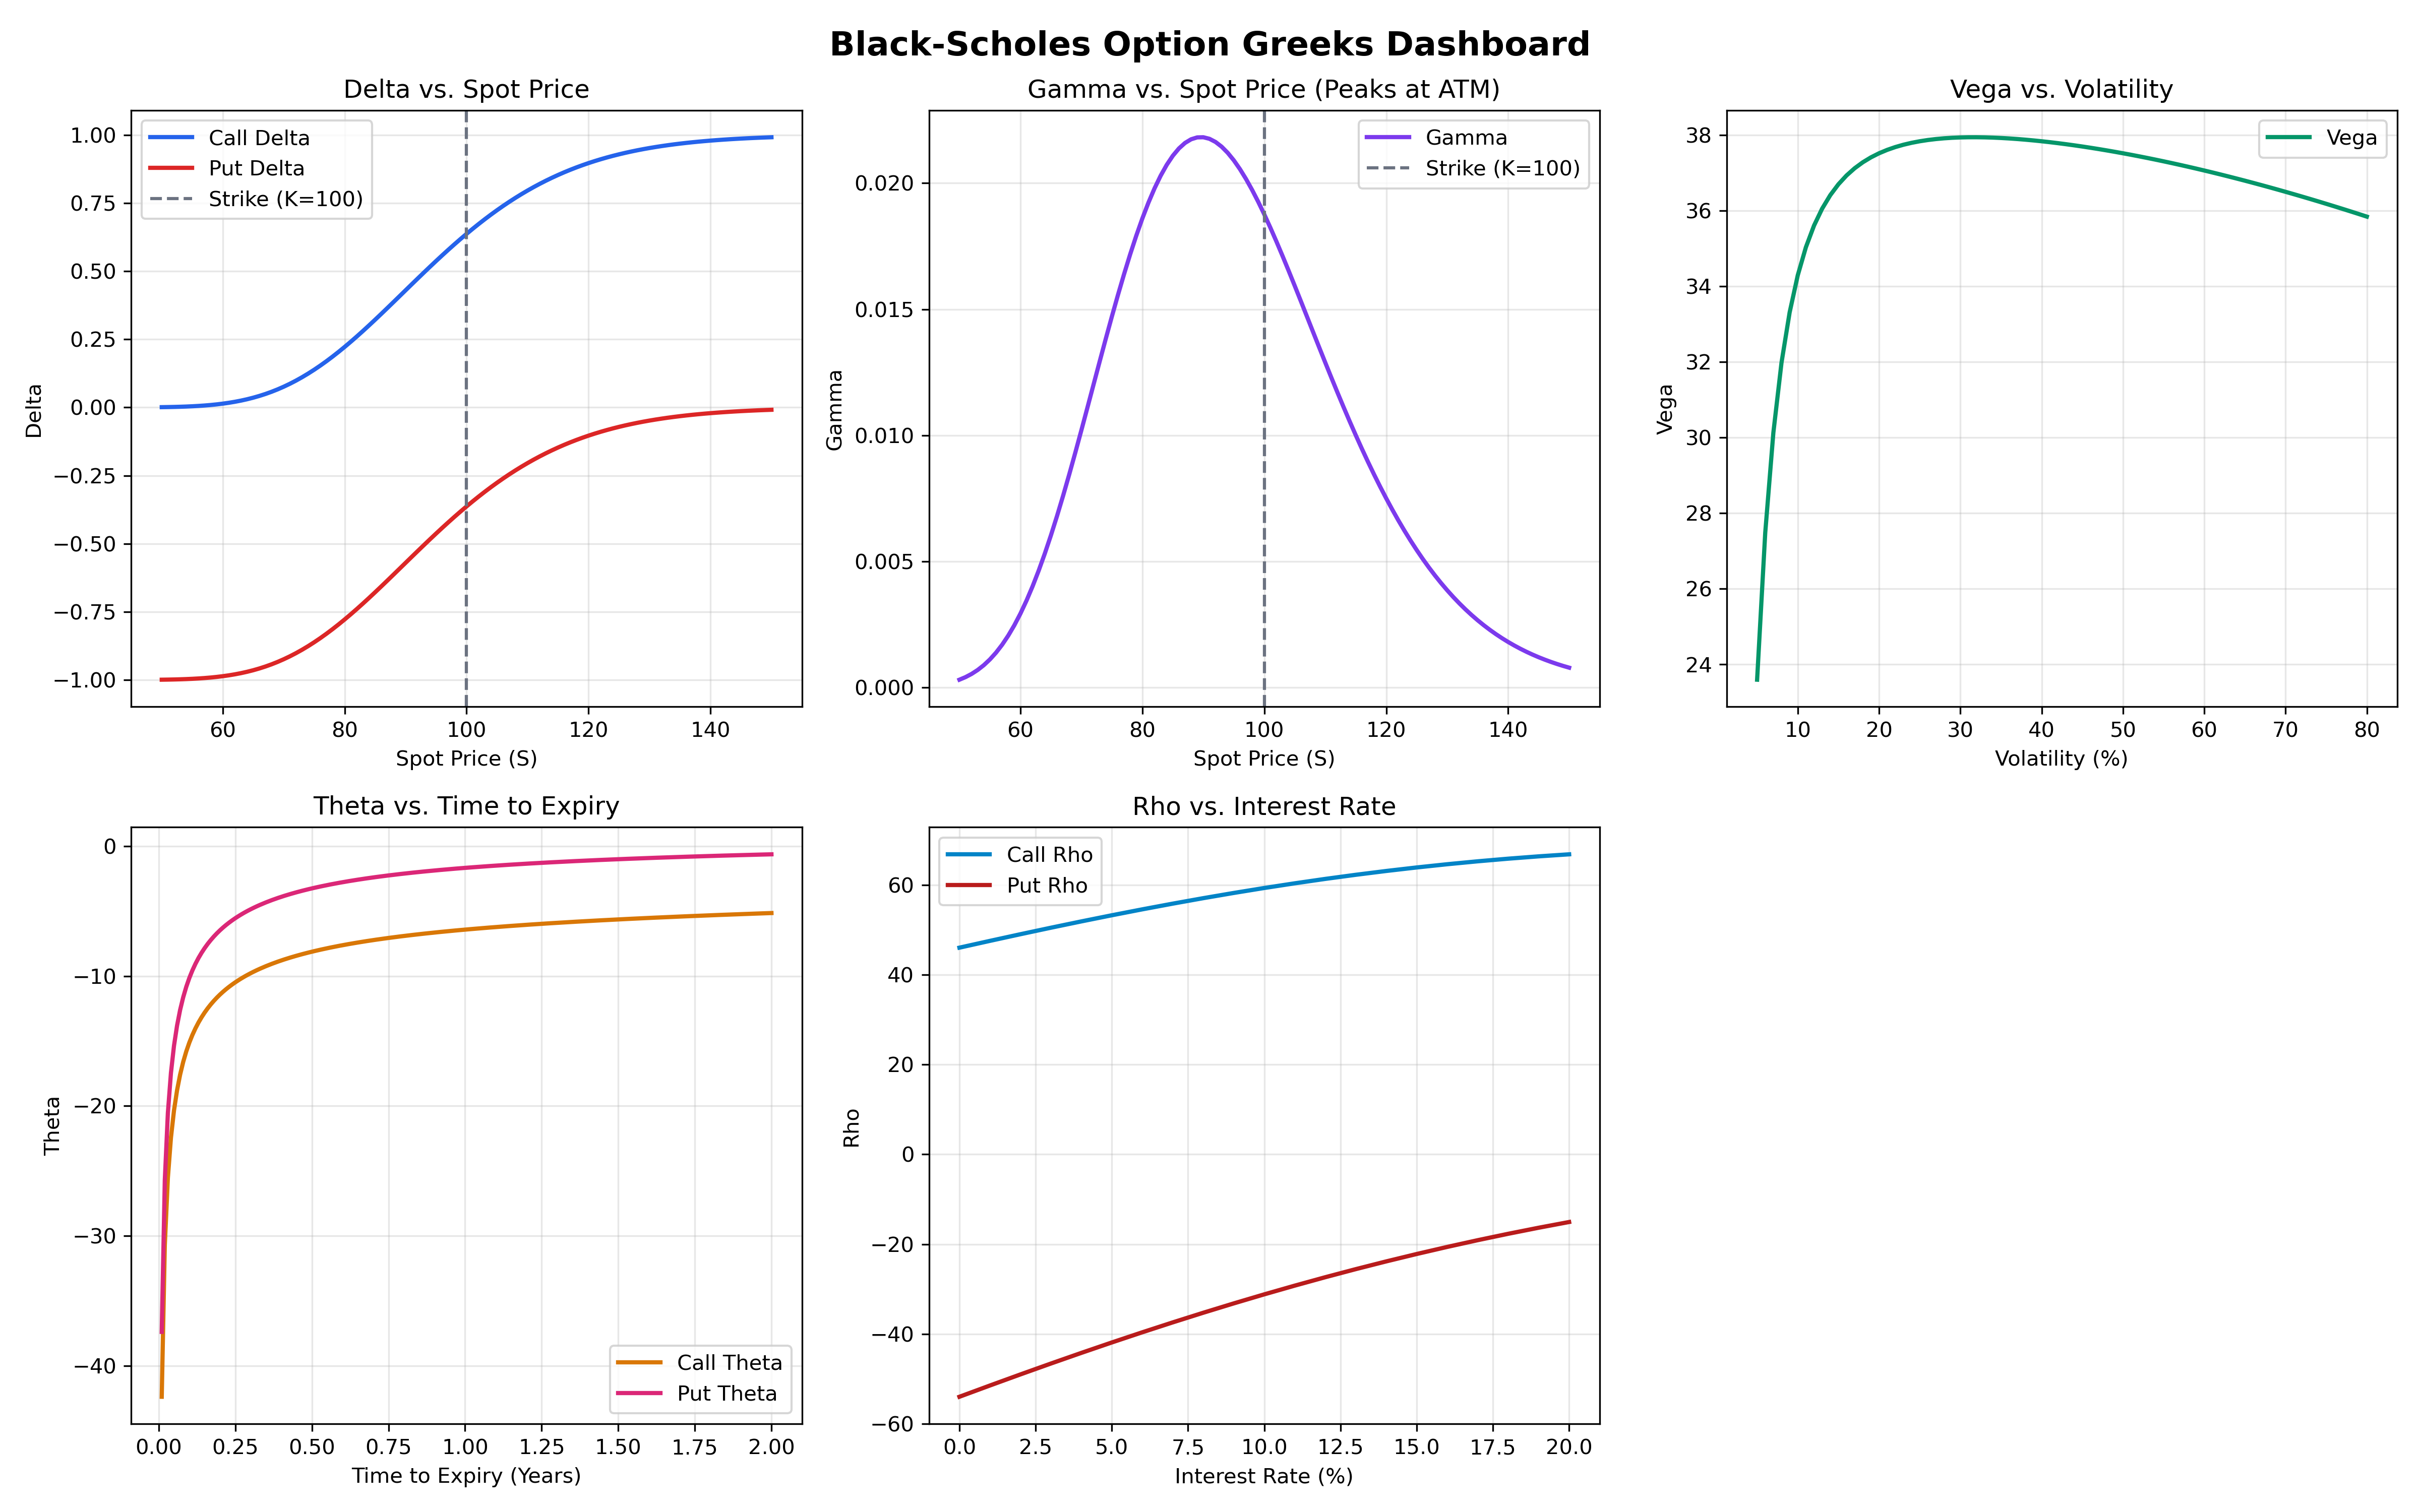
\includegraphics[width=0.82\textwidth]{greeks_dashboard.png}
  \caption{Interactive Greeks dashboard: Delta, Gamma, Theta, Vega, and Rho
    plotted as a function of spot price for all methods.
    All analytical Greeks are computed from closed-form Black-Scholes
    derivatives; neural Greeks are computed via automatic differentiation
    through the MLP.}
  \label{fig:dashboard}
\end{figure>

\subsection{Training Dynamics}

\begin{figure}[H]
  \centering
  \begin{subfigure}[t]{0.48\textwidth}
    \centering
    \includegraphics[width=\textwidth]{mlp_loss_curve.png}
    \caption{MLP training loss (MSE) over 100 epochs.
      Convergence is monotone; validation loss tracks training loss
      without divergence, confirming the model is not overfitting.}
    \label{fig:mlp_loss}
  \end{subfigure}\hfill
  \begin{subfigure}[t]{0.48\textwidth}
    \centering
    \includegraphics[width=\textwidth]{training_losses.png}
    \caption{VAE training losses (reconstruction + KL divergence)
      over 200 epochs. The $\beta$-weighted KL term stabilises the
      latent space, enabling smooth surface generation.}
    \label{fig:vae_loss}
  \end{subfigure}
  \caption{Training dynamics for MLP (left) and VAE (right).}
  \label{fig:losses}
\end{figure}

\subsection{Where Machine Learning Adds Value}

The results establish a clear boundary for where machine learning architectures
provide genuine value versus where they fall short of classical alternatives.
None of the three deep learning methods tested outperform Black-Scholes on
overall MAE when both are applied to vanilla European call pricing with
available market IV.
This is the correct null result for an honest benchmarking study.

However, the deep learning methods solve structurally different problems:
\begin{itemize}[leftmargin=1.5em]
  \item \textbf{VAE:} Achieves a smooth, arbitrage-consistent IV surface
    (range 0.205–0.364) reconstructed from sparse market quotes, enabling
    pricing at strikes and tenors where no market quote exists---a capability
    that classical interpolation cannot guarantee to be free of calendar-spread
    or butterfly arbitrage.
  \item \textbf{LSTM-BS:} Embeds temporal information from 60-day historical
    return and VIX sequences into the vol forecast, providing pricing that is
    responsive to recent market regime without requiring a full recalibration
    event.
  \item \textbf{MLP:} When operating in-distribution, achieves sub-millisecond
    throughput for large batch pricing jobs, orders of magnitude faster than
    Monte Carlo.
\end{itemize}

These represent structural advantages in specific operational contexts, not
improvements in point accuracy on vanilla European options---a distinction
essential for the correct interpretation of these results.

% ═══════════════════════════════════════════════════════════════════════════════
\section{Discussion and Limitations}
\label{sec:discussion}
% ═══════════════════════════════════════════════════════════════════════════════

\subsection{Discussion}

Our benchmarking exercise yields four concrete takeaways for practitioners.

\textbf{1. Smile-consistency is a qualitative not a quantitative advantage.}
The Heston model is ranked fourth on MAE yet is uniquely correct on the shape
of the pricing surface.
A desk trading skew-sensitive instruments—barrier options, risk reversals,
variance swaps—must use a smile-consistent model regardless of its raw-MAE
rank on vanilla calls.

\textbf{2. Deep learning is a surface interpolation tool, not a vanilla pricer.}
On in-distribution vanilla pricing, a modern GPU can evaluate Black-Scholes
for $10^6$ options in under a second; no neural network improves on this
throughput-accuracy tradeoff.
The VAE's value is not in the final option price it produces but in the
smooth, no-arbitrage IV surface it reconstructs from sparse quotes---a problem
that linear or spline interpolation cannot solve guaranteedly.

\textbf{3. Temporal volatility structure matters.}
The LSTM-BS hybrid's consistent underperformance at ATM reveals that a scalar
vol forecast, however sophisticated the time-series model, cannot substitute
for a cross-sectional IV surface.
Future architectures should emit a full $\hat{\sigma}(K, T)$ function, not a
scalar, to exploit the LSTM's genuine advantage in regime detection.

\textbf{4. Training domain specification is decisive for MLP accuracy.}
The MLP's catastrophic degradation (MAE \$6.66) on SPY at \$736.70 after
training on \$[50, 150] is entirely avoidable.
Training on normalised log-moneyness features would eliminate this
domain-shift sensitivity entirely, a finding that should be standard practice
in any production neural pricer.

\subsection{Limitations}

Four limitations merit attention.

\begin{enumerate}
  \item \textbf{Flat-vol deep learning inputs.}
    All deep learning models were applied with a single-sigma volatility input.
    A model emitting a full strike-dependent $\sigma(K, T)$ surface would
    materially improve LSTM-BS and MLP performance across all buckets.
  \item \textbf{MLP training domain mismatch.}
    The MLP was trained on synthetic spot prices in \$[50, 150] and deployed on
    SPY at \$736---a domain shift the linear homogeneity scaling only partially
    mitigated.
    Training on log-moneyness features would eliminate this sensitivity.
  \item \textbf{European-only evaluation.}
    The evaluation is restricted to European-exercise call options.
    American puts, where early-exercise premiums are material, would produce a
    different ranking in which the CRR tree's structural advantage over
    Black-Scholes becomes significant.
  \item \textbf{Fixed Heston parameters.}
    The Heston evaluation uses global skew parameters ($\kappa=2$,
    $\sigma_v=0.3$, $\rho=-0.7$) rather than per-option calibration.
    A full nonlinear calibration would substantially reduce Heston's ITM
    and Deep ITM errors at the cost of increased computational complexity.
\end{enumerate}

% ═══════════════════════════════════════════════════════════════════════════════
\section{Conclusion}
\label{sec:conclusion}
% ═══════════════════════════════════════════════════════════════════════════════

This paper presented a reproducible, end-to-end comparison of seven options
pricing methodologies—three classical, one stochastic volatility model, and
three deep learning—evaluated on 200~live SPY call options across the full
moneyness spectrum.

The central finding is that when all methods are supplied with market-implied
volatility, the classical GBM trio (Black-Scholes, CRR Binomial, Monte Carlo)
achieves nearly identical accuracy (MAE spread of \$0.002), with Black-Scholes
dominating on speed at 0.01~ms per option.
The Heston stochastic volatility model achieves MAE \$1.04---fourth-best
overall---but is the only method that structurally generates a non-flat implied
volatility smile: negative spot-vol correlation ($\rho=-0.7$) produces the
canonical equity left skew, with IV ranging from 17.3\% (OTM calls) to
23.0\% (ITM calls) versus the 20\% flat line used by all GBM pricers.

Deep learning models do not improve point accuracy on vanilla European calls:
the best deep learning result (LSTM-BS, MAE \$1.05) is 16\% worse than the
best classical result (Black-Scholes, MAE \$0.91).
The correct interpretation is not that deep learning fails at option pricing,
but that it solves different problems---the VAE provides arbitrage-consistent
IV surface imputation, the LSTM provides regime-sensitive volatility forecasts,
and the MLP provides ultra-fast batch throughput when operating within its
training distribution.

Future work will extend this study in four directions:
(i)~full per-option Heston calibration via gradient-based optimisation;
(ii)~replacement of the scalar LSTM forecast with a neural SVI model that
directly parameterises the full IV surface;
(iii)~MLP training on actual ETF price history using normalised log-moneyness
features; and
(iv)~extension of the Monte Carlo engine to price path-dependent exotics
(barrier, Asian, lookback options) where neither Black-Scholes nor the binomial
tree applies analytically.

% ═══════════════════════════════════════════════════════════════════════════════
\section*{References}
% ═══════════════════════════════════════════════════════════════════════════════

\begingroup
\renewcommand{\section}[2]{}
\begin{thebibliography}{99}

\bibitem[Black and Scholes(1973)]{BlackScholes1973}
  Black, F., \& Scholes, M. (1973).
  The pricing of options and corporate liabilities.
  \textit{Journal of Political Economy}, \textbf{81}(3), 637--654.

\bibitem[Boyle(1977)]{Boyle1977}
  Boyle, P. P. (1977).
  Options: A Monte Carlo approach.
  \textit{Journal of Financial Economics}, \textbf{4}(3), 323--338.

\bibitem[Cox, Ross, and Rubinstein(1979)]{CRR1979}
  Cox, J. C., Ross, S. A., \& Rubinstein, M. (1979).
  Option pricing: A simplified approach.
  \textit{Journal of Financial Economics}, \textbf{7}(3), 229--263.

\bibitem[Gatheral(2006)]{Gatheral2006}
  Gatheral, J. (2006).
  \textit{The Volatility Surface: A Practitioner's Guide}.
  Wiley Finance.

\bibitem[Glasserman(2004)]{Glasserman2004}
  Glasserman, P. (2004).
  \textit{Monte Carlo Methods in Financial Engineering}.
  Springer.

\bibitem[Gross, Kruger, and Toerien(2025)]{GrossKruger2025}
  Gross, R., Kruger, A., \& Toerien, F. (2025).
  A comparative analysis of artificial neural networks and classical option
  pricing models.
  \textit{Journal of Computational Finance}, forthcoming.

\bibitem[Heston(1993)]{Heston1993}
  Heston, S. L. (1993).
  A closed-form solution for options with stochastic volatility with
  applications to bond and currency options.
  \textit{The Review of Financial Studies}, \textbf{6}(2), 327--343.

\bibitem[Hochreiter and Schmidhuber(1997)]{Hochreiter1997}
  Hochreiter, S., \& Schmidhuber, J. (1997).
  Long short-term memory.
  \textit{Neural Computation}, \textbf{9}(8), 1735--1780.

\bibitem[Kingma and Welling(2013)]{KingmaWelling2013}
  Kingma, D. P., \& Welling, M. (2013).
  Auto-encoding variational Bayes.
  \textit{arXiv preprint arXiv:1312.6114}.

\bibitem[Ruf and Wang(2020)]{RufWang2020}
  Ruf, J., \& Wang, W. (2020).
  Neural networks for option pricing and hedging: A literature review.
  \textit{Journal of Computational Finance}, \textbf{24}(1), 1--45.

\bibitem[Shvimer and Zhu(2024)]{ShvimerZhu2024}
  Shvimer, L., \& Zhu, W. (2024).
  Hybrid neural network option pricing model.
  \textit{arXiv preprint arXiv:2502.15757}.

\bibitem[Zheng et al.(2025)]{Zheng2025}
  Zheng, S., et al. (2025).
  Neural jumps: Learning jump-diffusion processes for option pricing.
  \textit{arXiv preprint}.

\end{thebibliography}
\endgroup

\end{document}
